\section{Proposed AMECF Architecture}
\label{sec:amecf}

\subsection{Architecture Overview}
The \textbf{AMECF} (\textbf{A}daptive \textbf{M}ulti-\textbf{E}ntity \textbf{C}ontext \textbf{F}usion) model leverages a Heterogeneous Graph Transformer (HGT)~\cite{hu2020heterogeneous} backbone designed to handle multi-type node feature spaces and disparate relation types without requiring manual meta-path engineering. The neural workflow consists of: (1) type-specific linear feature projections, (2) multi-head heterogeneous context fusion layers, (3) residual LayerNorm aggregations, and (4) an account classification head.

\begin{figure*}[t]
\centering
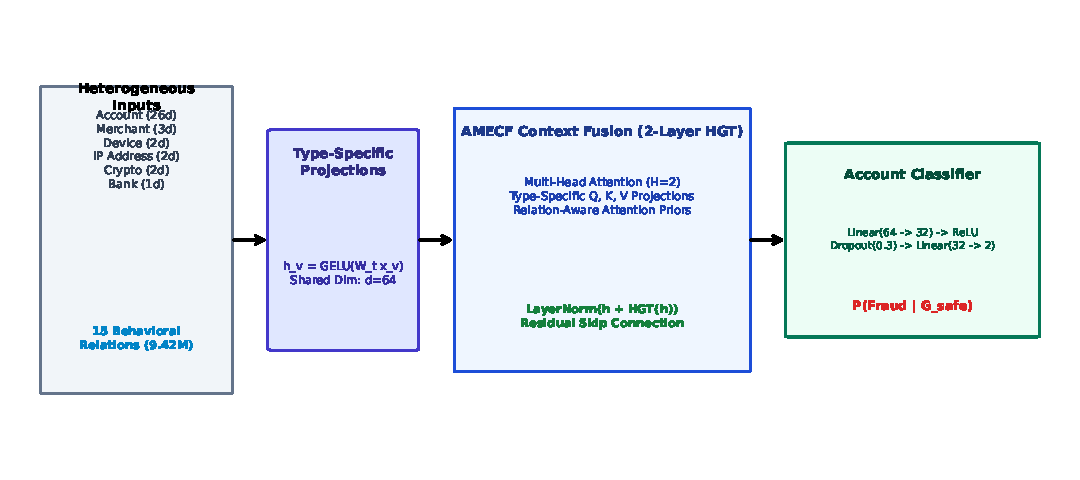
\includegraphics[width=0.92\textwidth]{figures/fig3_model_architecture.pdf}
\caption{Detailed neural architecture of the proposed Adaptive Multi-Entity Context Fusion (AMECF) network, illustrating type-specific input projections, multi-head heterogeneous attention computation over 15 behavioral relation types, residual LayerNorm skip connections, and the target account classification head.}
\label{fig:model_arch}
\end{figure*}

\subsection{Type-Specific Feature Projection}
Because entity types possess heterogeneous feature dimensionality ($d_{\text{account}} = 26$, $d_{\text{merchant}} = 3$, $d_{\text{atm}} = 2$, $d_{\text{device}} = 2$, $d_{\text{ip}} = 2$, $d_{\text{bank}} = 1$, etc.), each node type $\tau \in \mathcal{T}_v$ is first projected into a unified hidden embedding space of dimension $d_h = 64$:
\begin{equation}
    \mathbf{h}_v^{(0)} = \text{GELU}\left(\mathbf{W}_{\phi(v)}^{\text{proj}} \mathbf{x}_v + \mathbf{b}_{\phi(v)}^{\text{proj}}\right), \quad \forall v \in \mathcal{V}
\end{equation}
where $\mathbf{W}_\tau^{\text{proj}} \in \mathbb{R}^{d_h \times d_\tau}$ and $\mathbf{b}_\tau^{\text{proj}} \in \mathbb{R}^{d_h}$ are learnable projection parameters for node type $\tau$.

\subsection{Heterogeneous Attention Mechanism}
For an edge $e = (s, r, t)$ with relation type $r = (\phi(s), \rho, \phi(t))$, the $m$-th attention head computes a multi-relational attention score between target node $t$ and source neighbor $s$:
\begin{equation}
    \mathbf{Q}^{(m)}(t) = \mathbf{W}_{\phi(t)}^{Q, m} \mathbf{h}_t^{(l-1)}, \quad \mathbf{K}^{(m)}(s) = \mathbf{W}_{\phi(s)}^{K, m} \mathbf{h}_s^{(l-1)}
\end{equation}
\begin{equation}
    \alpha^{(m)}(s, r, t) = \frac{\mathbf{Q}^{(m)}(t) \mathbf{R}_{\psi(e)}^{\text{att}, m} (\mathbf{K}^{(m)}(s))^\top}{\sqrt{d_h / M}}
\end{equation}
where $\mathbf{W}_\tau^{Q, m}, \mathbf{W}_\tau^{K, m} \in \mathbb{R}^{\frac{d_h}{M} \times d_h}$ are type-specific Query and Key projection weights, $\mathbf{R}_r^{\text{att}, m} \in \mathbb{R}^{\frac{d_h}{M} \times \frac{d_h}{M}}$ is a relation-specific attention matrix capturing semantic correlation, and $M = 2$ is the number of attention heads.

The attention weights across all neighbors $\mathcal{N}(t)$ are normalized via a relation-aware softmax:
\begin{equation}
    a(s, r, t) = \underset{\forall s \in \mathcal{N}(t)}{\text{Softmax}} \left( \bigoplus_{m=1}^M \alpha^{(m)}(s, r, t) \cdot \mu_r \right)
\end{equation}
where $\mu_r \in \mathbb{R}$ represents a learnable relation significance scalar prior.

\subsection{Message Passing \&  Residual LayerNorm}
The message extracted from source neighbor $s$ is computed via:
\begin{equation}
    \mathbf{M}^{(m)}(s, r, t) = \mathbf{W}_{\phi(s)}^{V, m} \mathbf{h}_s^{(l-1)} \mathbf{R}_{\psi(e)}^{\text{msg}, m}
\end{equation}
Messages are aggregated across all incoming relations $\mathcal{E}(t)$ and updated with residual normalization:
\begin{equation}
    \tilde{\mathbf{h}}_t^{(l)} = \bigoplus_{m=1}^M \left( \sum_{s \in \mathcal{N}(t)} a^{(m)}(s, r, t) \mathbf{M}^{(m)}(s, r, t) \right)
\end{equation}
\begin{equation}
    \mathbf{h}_t^{(l)} = \text{LayerNorm}\left( \mathbf{h}_t^{(l-1)} + \mathbf{W}_{\phi(t)}^{\text{up}} \tilde{\mathbf{h}}_t^{(l)} \right)
\end{equation}
The full AMECF model stacks $L = 2$ heterogeneous attention layers, allowing target accounts to aggregate contextual signals from 2-hop entity neighborhoods (e.g., account $\to$ device $\to$ linked accounts, account $\to$ merchant $\to$ crypto gateway).

\subsection{Account Classification Head}
The final representation of account node $u \in \mathcal{V}_{\text{acc}}$ after layer $L$ is passed to an MLP classification head with dropout ($p = 0.3$):
\begin{equation}
    \hat{y}_u = \text{Softmax}\left( \mathbf{W}_2 \cdot \text{ReLU}\left(\mathbf{W}_1 \mathbf{h}_u^{(L)} + \mathbf{b}_1\right) + \mathbf{b}_2 \right)
\end{equation}
where $\mathbf{W}_1 \in \mathbb{R}^{32 \times 64}$, $\mathbf{W}_2 \in \mathbb{R}^{2 \times 32}$.
